For the Portugal panel, we developed five graphs that we'll explain next:\\
First, after read the \verb!csv! file from our source, using the \texttt{reavtiveVal()} function, we construct a {\sf{reactive value}} with the information filtered to only have Portugal's data. After this,  with a few skills in logic and programming, it's easier to work with the resultant dataset. \\
\\
In short, at this moment we have a {\sf{reactive value}}  with information only from Portugal.\\
We will explain our developed plots, but only the first one will be fully described. The others are similar, so we will show only the way that we think and point some differences.

\subsubsection{People totally vaccinated by age and laboratory}

To make this plot, we started by examining the dataset relative to Portugal's data only, and realized that we needed to filter it by age group. At this stage, we create six new and filtered datasets, each one with a specific \verb!TargetGroup!. \\ 
Then,  we need to take each one of these newer datasets and filter them four times. This happens because, at this day, there are only four vaccines distributed in Portugal. \\ 
In this last step we also choose only two columns from the dataset: \verb!YearWeekISO! and \verb!FirstDose! or \verb!SecondDose!, depending on the vaccine. This means that, at this moment, we have twenty four ($6 \times 4 = 24$) simple datasets with all the information simplified that we need. \\
At the end, we create one data frame with all this data, and also other information such as: age Group, laboratory of the Vaccine, to be possible to arrange the plot later.
\\
The  diagram (\ref{fig:overview2}) shows the complexity of the data processing.

\begin{figure}[h!]
\centering
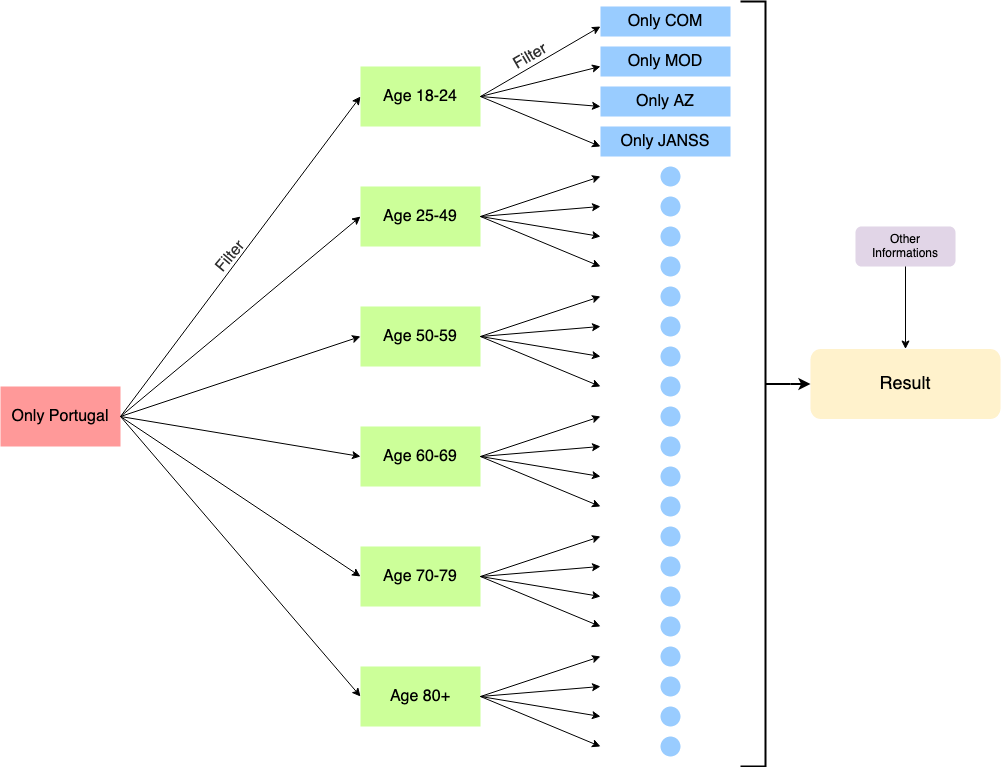
\includegraphics[width=300pt,trim=10 0 0 -10mm]{images/coiso2.png}
\caption{Data processing overview}
\label{fig:overview2}
\end{figure}

The \verb!Result! that we see in this figure, it's a reactive value with the data frame that will be used to render the plot.\\ This scheme, it's very similar in all data processing.\\

To render this plot, we use the \texttt{renderPlot()} function and save the result on a variable that will be the output displayed in the application. This behavior it's the same in all plots that we will show.\\
In this case, we call the data frame created at the end of the data processing, and we use the \texttt{ggplot()} function to create the plot. Then, as we want to display our plot in bars, with some visible information, we use the \texttt{geom\_bar()} and \texttt{geom\_text()} functions. We have some attributes in the \texttt{ggplot()} function that lets us handle with some theme and aesthetic details.
\\ To be easier to understand, consider this:
\begin{itemize}
    \item The 'Result' data frame will have the following structure:
    \begin{center}
        \begin{tabular}{ |c|c|c| } 
             \hline
             \textbf{{Idade}} & \textbf{Vac} & \textbf{Doses} \\ \hline
             Age group & Name of Laboratory/Vaccine & Number of people vaccinated \\  
             ... & ... & ...\\
             \hline
        \end{tabular}
    \end{center}
\end{itemize} 

Next we will show the actual code to render the plot that we want:\\

\begin{verbatim}
    output$myPlotPais <- renderPlot({
  
  res <- myReactiveDataPais() # Save the data set in the variable 'res'
  ggplot(res, aes(x= Vac, y=Doses, fill = Idades)) + 
    geom_bar(stat='identity', position = position_dodge())+
    geom_text(aes(label = Doses), vjust = -0.2,
              position = position_dodge(0.9), size = 3) +
    theme(
      axis.text.x = element_text(vjust = 1, size = 10,),
      axis.text.y = element_blank(),
      axis.ticks.y = element_blank(),
      axis.title = element_text(face="bold", size=18),
      title = element_text(size = 20),
      panel.grid = element_blank(),
      panel.background = element_rect(fill ="#ffffff")
    ) + 
    guides(fill= guide_legend(title = "Faixas etárias:")) +
    xlab('') + 
    ylab('') 
  
})
\end{verbatim}

As you can see, this is a good example to show how we render plots, after the data processing. In the future, this example will not be displayed here again. \\
The result of this plot  (\ref{fig:ages-vac}) is the following:\\

\begin{figure}[H]
\centering
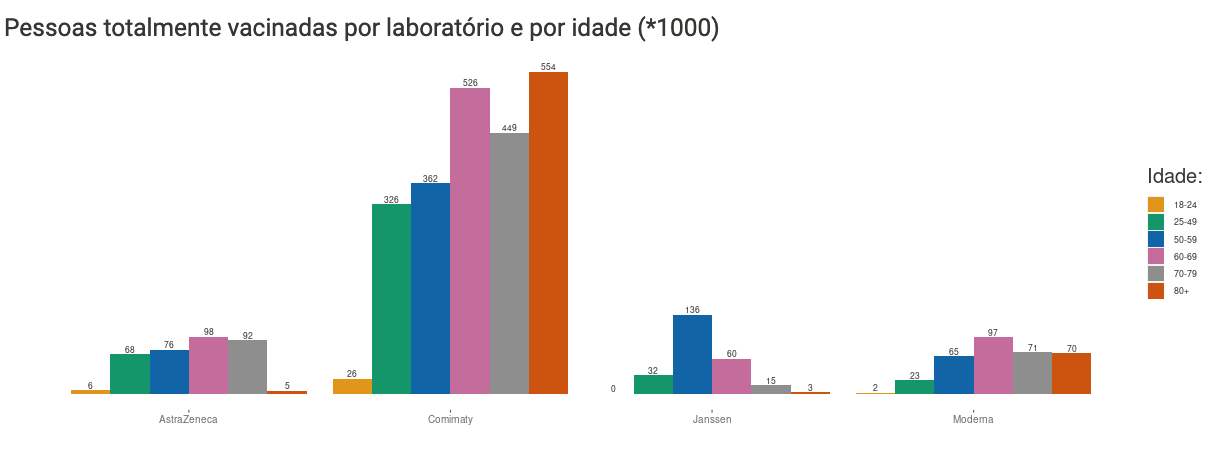
\includegraphics[width=400pt,trim=10 0 0 -10mm]{images/coiso3.png}
\caption{Plot of people totally vaccinated by age and laboratory}
\label{fig:ages-vac}
\end{figure}


\subsubsection{People totally vaccinated by age, by week}
This is a time plot segmented by age,  to visualise the behaviour of the number of vaccinated people,  week by week, in each group age.\\
Since there are much information in this graphic, we choose to give the user options to see the data.\\
The user can choose if he wants to see, or not, the value in each age group by week. %It's possible to choose how many age groups want  display simultaneously in the plot. This makes it possible for the user to compare as many as he wants.\\
\\
It is possible to choose how many age groups you want to display simultaneously on the chart. This allows the user to compare those vaccinated according to age.
\\
As mention earlier, the data processing it's pretty much similar, and this is one of those cases. Such as the previous graphic, we will filter the data set that have information only from Portugal, creating new data sets with specific information that we need to move on. In each one of these data sets, we need to preserve the week of vaccination and, for each week, sum all the people vaccinated by age group.
After the data processing, the result should be something with this structure:\\

    \begin{center}
        \begin{tabular}{ |c|c|c|c|c| } 
             \hline
             \textbf{\textit{Datas}} & \textbf{\textit{Vacinados18\_24}} & \textbf{\textit{Vacinados25\_49}} & \textbf{\textit{Vacinados\_ageGroup}} & ...\\ \hline
             Week$_n$ & \texttt{int} & \texttt{int} & \texttt{int} & ... \\  
             \hline
             Week$_{n+1}$ & \texttt{int} & \texttt{int} & \texttt{int} & ... \\  
             \hline 
             ... & ... & ... & ... & ...\\
             \hline
        \end{tabular}
    \end{center}

To render this plot, the process is the same as the previous plot, except that, in this one, we'll save the \texttt{ggplot()} in a variable (this is a feature of the graphics produced with \verb!ggplot2!). This makes possible that, in the future, we can add more information to this plot.\\
This information it's input passed by the user. When he chooses some option, our plot will update, adding or removing the information that he chose. Next we'll show different ways to observe the plot (\ref{fig:ages-vac-1})

\begin{figure}[H]
\centering
%width=\textwidth
%width=350pt,trim=10 0 0 -10mm
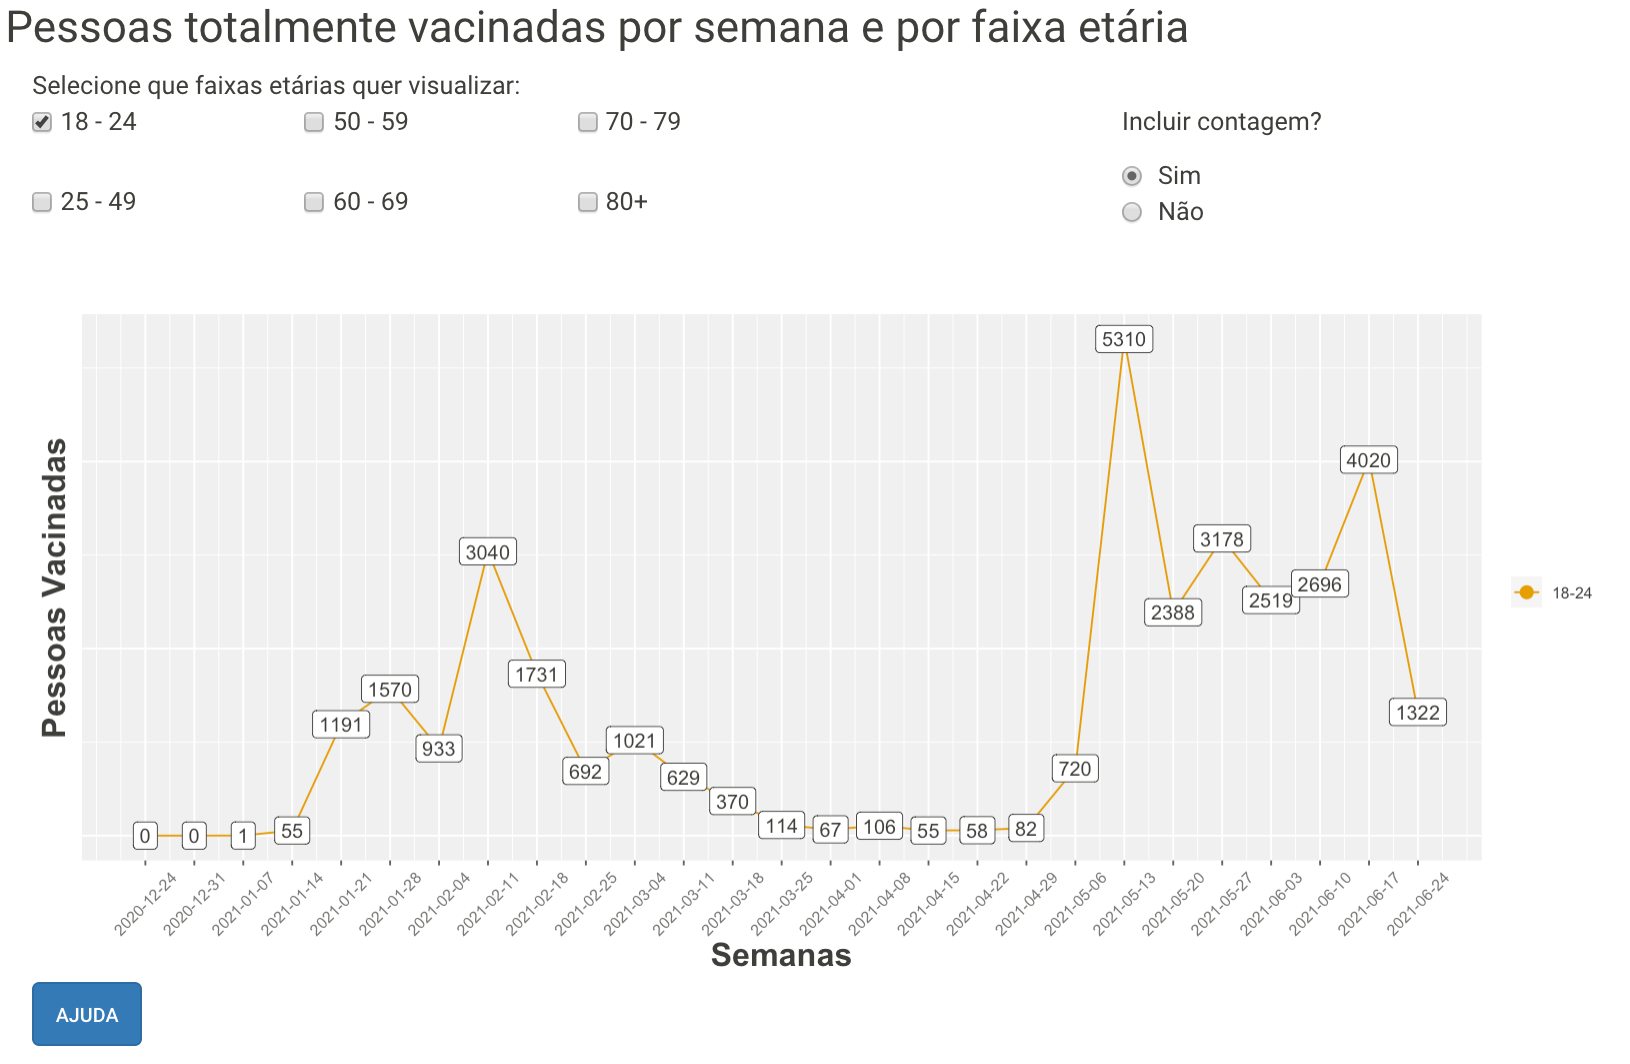
\includegraphics[width=\textwidth]{images/p1.png}
\caption{Plot with count, of the age group 18-24}
\label{fig:ages-vac-1}
\end{figure}
 As you can see, in the graphic (\ref{fig:ages-vac-1}), we include count and the age group selected is only 18-24.\\

\begin{figure}[H]
\centering
%width=350pt,trim=10 0 0 -10mm
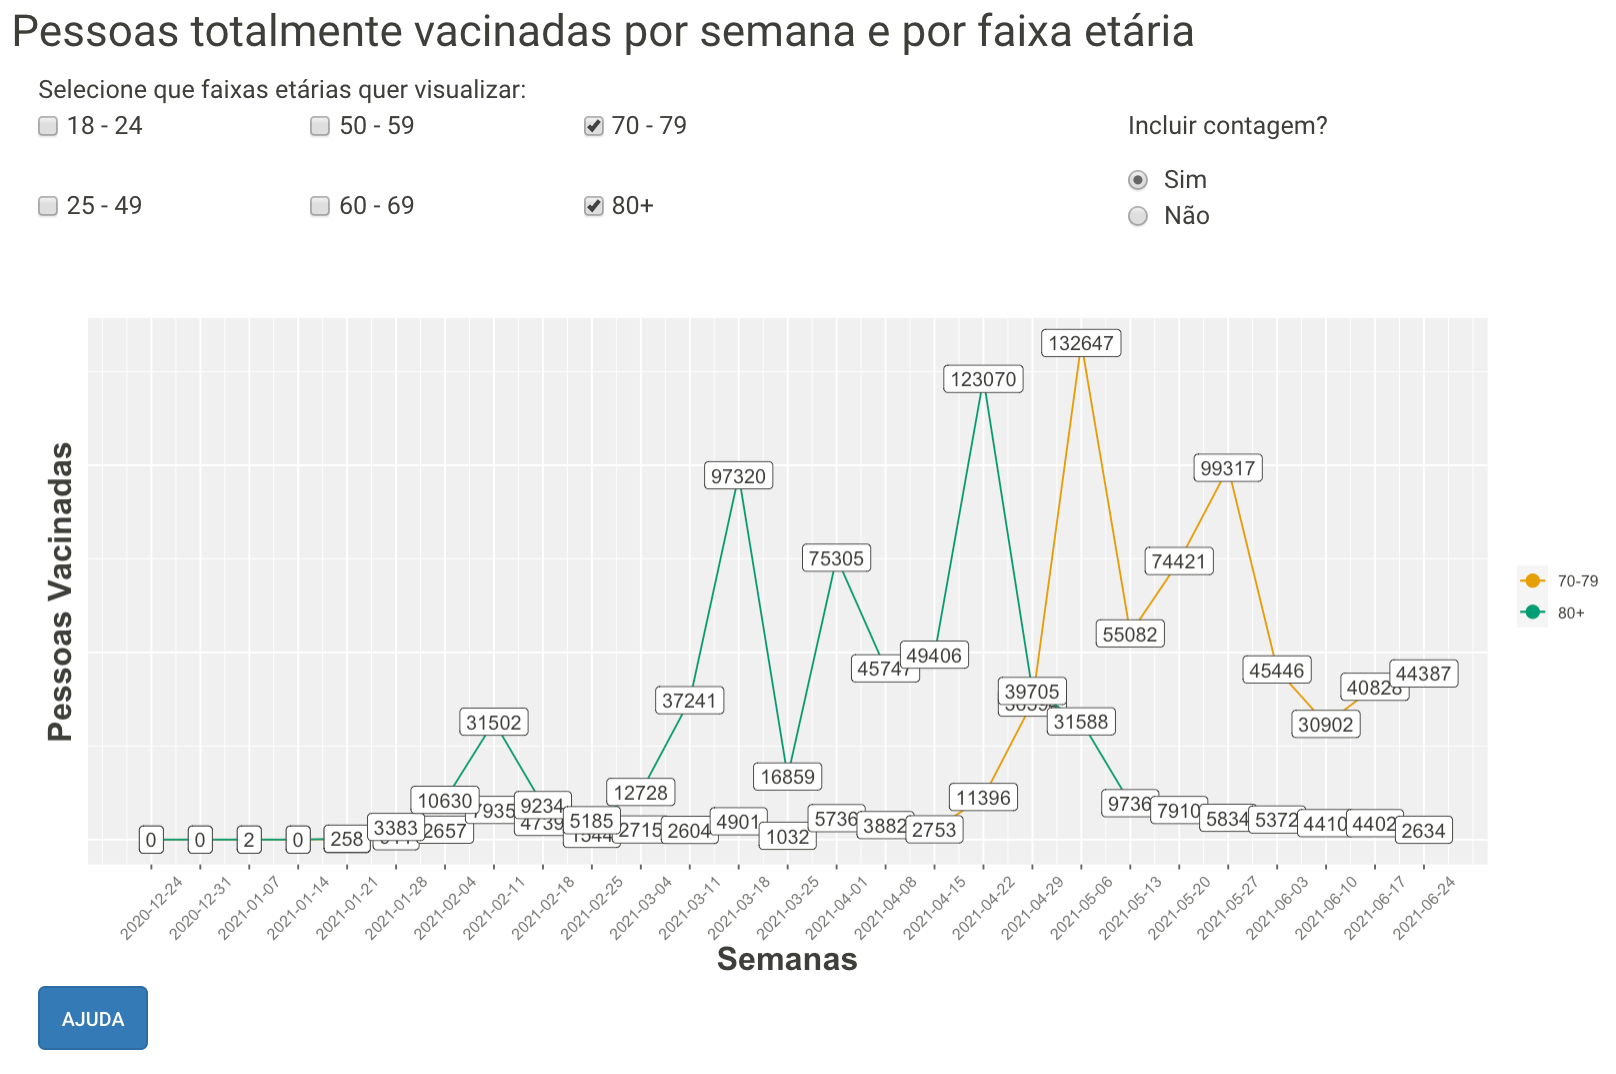
\includegraphics[width=\textwidth]{images/p2.png}
\caption{Plot with count, of the age groups 70-79 and 80+}
\label{fig:ages-vac-3}
\end{figure}
In the graphic (\ref{fig:ages-vac-3}), we include count and the age groups selected are 70-79 and 80+. This makes possible for the user to compare information.\\
As you can see, if you want to have an intuitive view of the evolution in every week, with the values displayed turns out to be hard.\\
That's the reason to give the option without the count. As shown next, Figure \ref{fig:ages-vac-4},  it's possible even to see some information justified by the vaccination plane and more. 

\begin{figure}[H]
\centering
%width=350pt,trim=10 0 0 -10mm
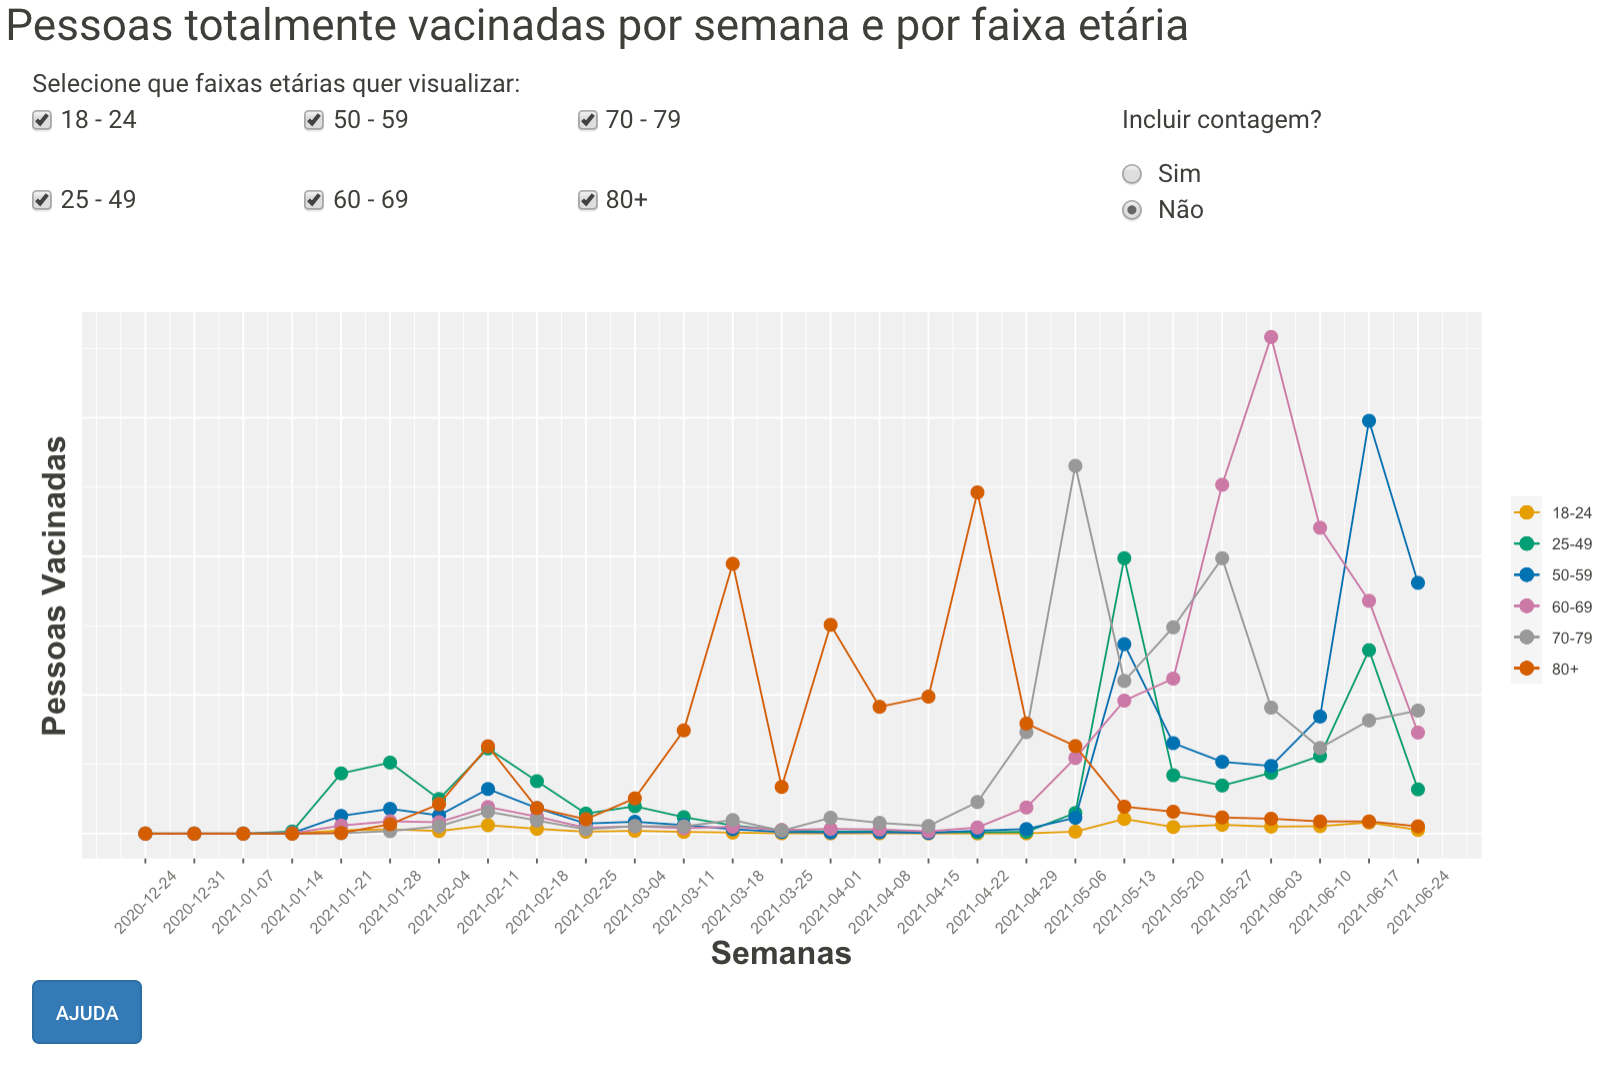
\includegraphics[width=\textwidth]{images/p4.png}
\caption{Plot without count, of all age groups}
\label{fig:ages-vac-4}
\end{figure}

\subsubsection{People totally vaccinated by region, by week}

This one it's exactly the same as the one before, with the difference of filter the total of people vaccinated by region, instead of group age.

\subsubsection{Vaccines administered by laboratory}

In terms of data processing, there's not any new way to do things. The result will be the shown in (\ref{fig:ages-vac-5}).\\
\begin{figure}[H]
\centering
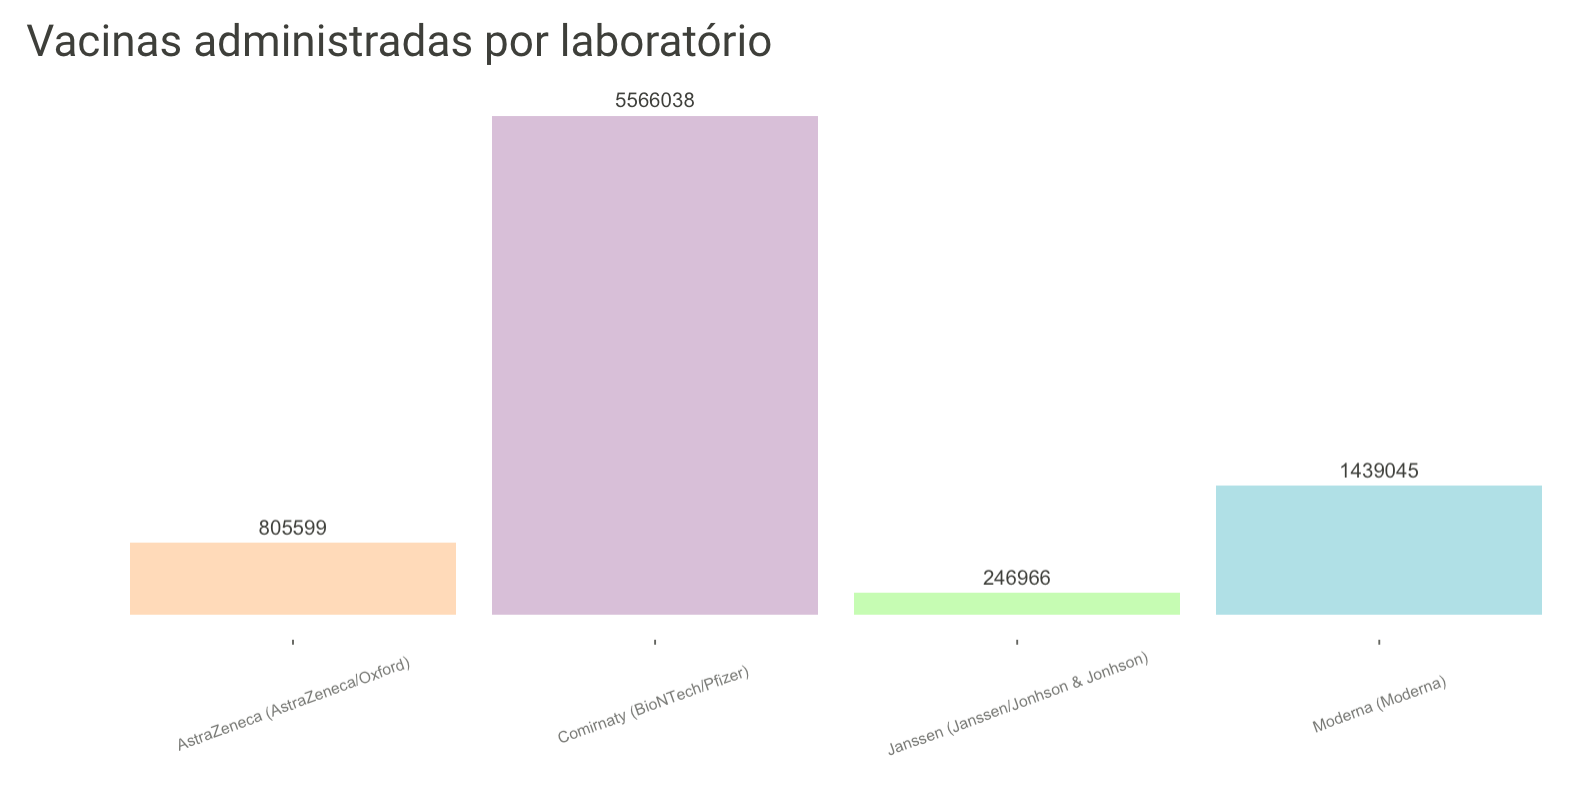
\includegraphics[width=350pt,trim=10 0 0 -10mm]{images/p5.png}
\caption{Plot with the number of administered vaccines by laboratory}
\label{fig:ages-vac-5}
\end{figure}

In this plot, all the administered doses are referent of the first and second dose of each vaccine.

\subsubsection{Percentages of vaccinated and unvaccinated people}

In this graphic, the data process is similar to the previous graphics with the exception that now, we want to work with percentages. With this in mind, we know the population of Portugal and with simple math it's easy to create the reactive value to render the plot.\\
\\
This graphic (\ref{fig:ages-vac-6}) uses a function from another package ('waffle'), that allow the function \texttt{renderPlot()} to display the information in a waffle plot. 
\begin{figure}[H]
\centering
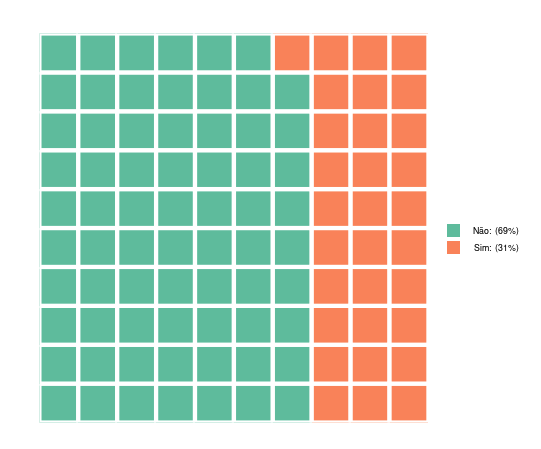
\includegraphics[width=350pt,trim=10 0 0 -10mm]{images/p6.png}
\caption{Plot with the percentages of vaccinated/unvaccinated people}
\label{fig:ages-vac-6}
\end{figure}
We choose to develop this plot this way, not only because, in our opinion, it looks good, but also to show that \textbf{ggplot2} can be very versatile.